\documentclass[hidelinks,12pt]{article}
\usepackage[left=0.25cm,top=1cm,right=0.25cm,bottom=1cm]{geometry}
%\usepackage[landscape]{geometry}
\textwidth = 20cm
\hoffset = -1cm
\usepackage[utf8]{inputenc}
\usepackage[spanish,es-tabla]{babel}
\usepackage[autostyle,spanish=mexican]{csquotes}
\usepackage[tbtags]{amsmath}
\usepackage{nccmath}
\usepackage{amsthm}
\usepackage{amssymb}
\usepackage{mathrsfs}
\usepackage{graphicx}
\usepackage{subfig}
\usepackage{standalone}
\usepackage[outdir=./Imagenes/]{epstopdf}
\usepackage{siunitx}
\usepackage{physics}
\usepackage{color}
\usepackage{float}
\usepackage{hyperref}
\usepackage{multicol}
%\usepackage{milista}
\usepackage{anyfontsize}
\usepackage{anysize}
%\usepackage{enumerate}
\usepackage[shortlabels]{enumitem}
\usepackage{capt-of}
\usepackage{bm}
\usepackage{relsize}
\usepackage{placeins}
\usepackage{empheq}
\usepackage{cancel}
\usepackage{wrapfig}
\usepackage[flushleft]{threeparttable}
\usepackage{makecell}
\usepackage{fancyhdr}
\usepackage{tikz}
\usepackage{bigints}
\usepackage{scalerel}
\usepackage{pgfplots}
\usepackage{pdflscape}
\pgfplotsset{compat=1.16}
\spanishdecimal{.}
\renewcommand{\baselinestretch}{1.5} 
\renewcommand\labelenumii{\theenumi.{\arabic{enumii}})}
\newcommand{\ptilde}[1]{\ensuremath{{#1}^{\prime}}}
\newcommand{\stilde}[1]{\ensuremath{{#1}^{\prime \prime}}}
\newcommand{\ttilde}[1]{\ensuremath{{#1}^{\prime \prime \prime}}}
\newcommand{\ntilde}[2]{\ensuremath{{#1}^{(#2)}}}

\newtheorem{defi}{{\it Definición}}[section]
\newtheorem{teo}{{\it Teorema}}[section]
\newtheorem{ejemplo}{{\it Ejemplo}}[section]
\newtheorem{propiedad}{{\it Propiedad}}[section]
\newtheorem{lema}{{\it Lema}}[section]
\newtheorem{cor}{Corolario}
\newtheorem{ejer}{Ejercicio}[section]

\newlist{milista}{enumerate}{2}
\setlist[milista,1]{label=\arabic*)}
\setlist[milista,2]{label=\arabic{milistai}.\arabic*)}
\newlength{\depthofsumsign}
\setlength{\depthofsumsign}{\depthof{$\sum$}}
\newcommand{\nsum}[1][1.4]{% only for \displaystyle
    \mathop{%
        \raisebox
            {-#1\depthofsumsign+1\depthofsumsign}
            {\scalebox
                {#1}
                {$\displaystyle\sum$}%
            }
    }
}
\def\scaleint#1{\vcenter{\hbox{\scaleto[3ex]{\displaystyle\int}{#1}}}}
\def\bs{\mkern-12mu}


\usepackage{apacite}
\title{Clase 05 - Funciones Gamma y Beta \\[0.3em]  \large{Matemáticas Avanzadas de la Física}\vspace{-3ex}}
\author{M. en C. Gustavo Contreras Mayén}
\date{ }
\begin{document}
\vspace{-4cm}
\maketitle
\fontsize{14}{14}\selectfont
\tableofcontents
\newpage

%Ref. Andrews (1998) Chapter 10. 2.2
\section{La función Gamma.}

Una de las funciones especiales más simples pero muy importantes es la función Gamma, que escribimos como $\Gamma (x)$. Aparece ocasionalmente por sí misma en aplicaciones físicas (principalmente en forma de alguna integral), pero gran parte de su importancia radica en su utilidad para desarrollar otras funciones como las \emph{funciones de Bessel} y las \emph{funciones hipergeométricas} que tienen una aplicación física más directa.
\par
La función Gamma tiene varias definiciones equivalentes, la mayoría de las cuales se deben a Euler. Para empezar, sin embargo, usamos la definición:
\begin{align}
\Gamma (x) = \lim_{n \to \infty} \, \dfrac{n!}{x (x + 1)(x + 2) \cdots (x + n)} \, n^{x}
\label{eq:ecuacion_02_01}
\end{align}
que en realidad se debió a C. Gauss (1777-1855). Si $x$ no es cero o un entero negativo, se puede demostrar que el límite (\ref{eq:ecuacion_02_01}) existe. Sin embargo, es evidente que $\Gamma (x)$ no se puede definir en $x = 0, -1, -2, \ldots$, ya que el límite se vuelve infinito para cualquiera de estos valores. Como consecuencia se tiene el siguiente teorema.

\begin{teo}\label{teorema_01_01}
Si $x = - n$ con $n = 0, 1, 2 \ldots$, entonces:
\begin{align*}
\abs{\Gamma (x)} \to \infty
\end{align*}
o de manera equivalente:
\begin{align*}
\dfrac{1}{\Gamma (-n)} = 0 \hspace{1.5cm} n = 0, 1, 2, \ldots
\end{align*}

Haciendo que $x = 1$ en la ec. (\ref{eq:ecuacion_02_01}), vemos que:
\begin{align*}
\Gamma (1) = \lim_{n \to \infty} \dfrac{n! \, n}{1 \cdot 2 \cdot 3 \cdots n (n + 1)} = \lim_{n \to \infty} \dfrac{n}{n + 1}
\end{align*}
de donde se obtiene un valor especial:
\begin{align}
\Gamma (1) = 1
\label{eq:ecuacion_02_02}
\end{align}
\end{teo}

Otros valores de $\Gamma (x)$ no se obtienen tan fácilmente, pero la sustitución de $x + 1$ por $x$ en la ec. (\ref{eq:ecuacion_02_01}) nos conduce a:
\begin{align*}
\begin{aligned}
\Gamma (x + 1) &= \lim_{n \to \infty} \dfrac{n! \, n^{x+1}}{(x + 1)(x + 2) \cdots (x + n)(x + n + 1)} = \\[0.5em]
&= \lim_{n \to \infty} \dfrac{n \, x}{x + n + 1} \, \lim_{n \to \infty} \dfrac{n! \, n^{x}}{x (x + 1) \ldots (x + n)}
\end{aligned}
\end{align*}
de donde se recupera la fórmula de recurrencia:
\begin{align}
\Gamma (x + 1) =  x \, \Gamma (x)
\label{eq:ecuacion_02_03}
\end{align}

La ecuación (\ref{eq:ecuacion_02_03}) es la relación funcional básica para la función Gamma; tiene la forma de una \emph{ecuación en diferencias}. Si bien muchas de las funciones especiales satisfacen alguna \emph{ecuación diferencial lineal}, se ha demostrado que la función Gamma no satisface ninguna ecuación diferencial lineal con coeficientes racionales.
\par
Se puede obtener una conexión directa entre la función Gamma y los factoriales a partir de las ecs. (\ref{eq:ecuacion_02_02}) y (\ref{eq:ecuacion_02_03}). Es decir, si combinamos estas relaciones, tenemos:
\begin{align*}
\Gamma (2) &= 1 \cdot \Gamma(1) = 1 \\[0.5em]
\Gamma (3) &= 2 \cdot \Gamma(2) = 2 \cdot 1 = 2! \\[0.5em]
\Gamma (4) &= 3 \cdot \Gamma(3) = 3 \cdot 2! = 3! \\[0.5em]
\vdots
\end{align*}
mediante inducción matemática se puede demostrar que:
\begin{align}
\Gamma (n + 1) = n! \hspace{1.5cm} n = 0, 1, 2, \ldots
\label{eq:ecuacion_02_04}
\end{align}
Así, la función Gamma es una generalización de la función factorial del dominio de los enteros positivos al dominio de todos los números reales (excepto como se indica en el Teorema \ref{teorema_01_01}).

\subsection{Representaciones integrales.}

La razón para usar la definición de límite como se indica en la ec. (\ref{eq:ecuacion_02_01}) de la función Gamma es que la define para valores negativos de $x$ así como para valores positivos.
\par
La función Gamma rara vez aparece en la forma dada por la ec. (\ref{eq:ecuacion_02_01}) en las aplicaciones. En cambio, surge con mayor frecuencia en la evaluación de ciertas integrales; por ejemplo, Euler pudo demostrar que:
\begin{align}
\Gamma (x) = \scaleint{6ex}_{\bs 0}^{\infty} e^{-t} \, t^{x- 1} \dd{t} \hspace{1.5cm} x > 0
\label{eq:ecuacion_02_05}
\end{align}

Esta \textbf{representación integral} de $\Gamma (x)$ es la forma más común en la que ahora se define la función Gamma. Dado que las integrales son bastante fáciles de manipular, a menudo se prefiere la expresión (\ref{eq:ecuacion_02_05}) que la (\ref{eq:ecuacion_02_01}) para desarrollar las propiedades de esta función. Sin embargo, la ecuación (\ref{eq:ecuacion_02_05}) es menos general que la (\ref{eq:ecuacion_02_01}), ya que la variable $x$ está restringida en la ec. (\ref{eq:ecuacion_02_05}) a valores positivos. Por último, notamos que la ec. (\ref{eq:ecuacion_02_05}) es una integral impropia, debido al límite infinito de integración y porque el factor $t^{x-1}$ tiende a infinito en $t = 0$ para valores de $x$ en el intervalo $0 < x < 1$. No obstante, la integral de la ec. (\ref{eq:ecuacion_02_05}) es \emph{uniformemente convergente} para todo a $a \leq x \leq b$, donde $0 < a \leq b < \infty$.
\par
Primero establezcamos la equivalencia de la ec. (\ref{eq:ecuacion_02_01}) y la ec. (\ref{eq:ecuacion_02_05}) para valores positivos de $x$. Para ello, establecemos:
\begin{align}
\begin{aligned}
F(x) &= \scaleint{6ex}_{\bs 0}^{\infty} e^{-t} \, t^{x- 1} \dd{t} = \\[0.5em]
&= \lim_{n \to \infty} \scaleint{6ex}_{\bs 0}^{\infty} \bigg( 1 - \dfrac{t}{n} \bigg)^{n} \, t^{x- 1} \dd{t} \hspace{1.5cm} x > 0
\end{aligned}
\label{eq:ecuacion_02_06}
\end{align}
recordemos que:
\begin{align}
e^{-t} = \lim_{n \to \infty} \bigg( 1 - \dfrac{t}{n} \bigg)^{n}
\label{eq:ecuacion_02_07}
\end{align}

Usando integración sucesiva por partes, después de hacer el cambio de variable $z = t/n$, encontramos que:
\begin{align}
\begin{aligned}[b]
F(z) &= \lim_{n \to \infty} n^{x} \, \scaleint{6ex}_{\bs 0}^{1} (1 - z)^{n} \, z^{x-1} \dd{z} = \\[0.5em]
&= \lim_{n \to \infty} n^{x} \bigg[ (1 - z)^{n} \, \dfrac{z^{x}}{x} \eval_{0}^{1} + \dfrac{n}{x} \scaleint{6ex}_{\bs 0}^{1} (1 - z)^{n-1} \, z^{x} \dd{z} \bigg] = \\[0.5em]
\vdots& \\[0.5em]
&= \lim_{n \to \infty} n^{x} \bigg[ \dfrac{n (n - 1) \cdots 2 \cdot 1}{x (x + 1) \cdots (x + n - 1)} \, \scaleint{6ex}_{\bs 0}^{1} z^{x+n-1} \dd{z} \bigg] = \\[0.5em]
&= \lim_{n \to \infty} \dfrac{n! \, n^{x}}{x (x + 1)(x + 2) \cdots (x + n)}
\end{aligned}
\label{eq:ecuacion_02_08}
\end{align}
y así hemos demostrado que:
\begin{align}
F(x) = \scaleint{6ex}_{\bs 0}^{\infty} e^{-t} \, t^{x-1} \dd{t} = \Gamma (x) \hspace{1.5cm} x > 0
\label{eq:ecuacion_02_09}
\end{align}

De la convergencia uniforme de la integral en la ec. (\ref{eq:ecuacion_02_05}) se sigue que $\Gamma (x)$ es una función continua para todo $x > 0$. Para investigar el comportamiento de $\Gamma (x)$ cuando $x$ se acerca al valor cero por la derecha, usamos la fórmula de recurrencia ec. (\ref{eq:ecuacion_02_03}) escrita en la forma:
\begin{align*}
\Gamma (x) = \dfrac{\Gamma (x + 1)}{x}
\end{align*}
Así, vemos que:
\begin{align}
\lim_{x \to 0^{+}} \Gamma (x) = \lim_{x \to 0^{+}} \dfrac{\Gamma (x + 1)}{x} \to +\infty
\label{eq:ecuacion_02_10}
\end{align}

Otra consecuencia de la convergencia uniforme de la integral que define a la $\Gamma (x)$ es que podemos derivar la función bajo el signo integral para obtener:
\begin{align}
\pderivada{\Gamma} (x) = \scaleint{6ex}_{\bs 0}^{\infty} e^{-t} \, t^{x-1} \, \ln x \dd{t} \hspace{1.5cm} x > 0
\label{eq:ecuacion_02_11}
\end{align}
así como:
\begin{align}
\sderivada{\Gamma} (x) = \scaleint{6ex}_{\bs 0}^{\infty} e^{-t} \, t^{x-1} \, \big( \ln x \big)^{2} \dd{t} \hspace{1.5cm} x > 0
\label{eq:ecuacion_02_12}
\end{align}

El integrando en la ec. (\ref{eq:ecuacion_02_12}) es positivo en todo el intervalo de integración y, por lo tanto, $\sderivada{\Gamma} (x) > 0$. Esto implica que la gráfica de $y = \Gamma (x)$ es \emph{cóncava hacia arriba} para todo $x > 0$. Mientras que los máximos y mínimos normalmente se encuentran al establecer la derivada de la función en cero, aquí hacemos la observación de que dado que $\Gamma (1) = \Gamma (2) = 1$ y $\Gamma (x)$ siempre es cóncava hacia arriba, la función Gamma tiene \emph{solo un mínimo} en el intervalo $x > 0$. Además, el mínimo ocurre en el intervalo $1 < x < 2$. La posición exacta del mínimo fue primero calculada por Gauss y resultó ser $x_{0} = 1.4616\ldots$ , lo que lleva al mínimo valor $\Gamma (x_{0}) = 0.8856\ldots$. Por último, de la continuidad de $\Gamma (x)$ y su concavidad, deducimos que:
\begin{align}
\lim_{x \to +\infty} \Gamma (x) \to +\infty
\label{eq:ecuacion_02_13}
\end{align}
Con este último resultado, hemos determinado las características fundamentales de la gráfica de la función $\Gamma (x)$ para $x > 0$, como se ve en la figura (\ref{fig:figura_02_01}).
\begin{figure}[H]
    \centering
    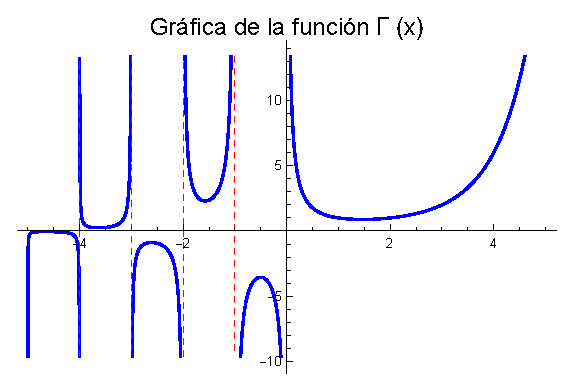
\includegraphics[scale=1]{Imagenes/Plot_Gamma_01.eps}
    \caption{Gráfica de la función Gamma en el intervalo $-5 < x < 5$.}
    \label{fig:figura_02_01}
\end{figure}

La función Gamma se define para valores positivos y negativos de $x$ por la ec. (\ref{eq:ecuacion_02_01}), aunque generalmente es más conveniente utilizar la fórmula de recurrencia (\ref{eq:ecuacion_02_03}) cuando se trata de valores negativos. Por ejemplo, si $x$ está en el rango $-1 < x < 0$, reescribimos la ec. (\ref{eq:ecuacion_02_03}) como:
\begin{align}
\Gamma (x) = \dfrac{\Gamma (x + 1)}{x} \hspace{1.5cm} x > -1, \hspace{0.5cm} x \neq 0
\label{eq:ecuacion_02_14}
\end{align}
y usamos el lado derecho para fines de cálculo. También usando la ec. (\ref{eq:ecuacion_02_14}), obtenemos los límites izquierdo y derecho:
\begin{align}
\lim_{x \to 0^{-}} \Gamma (x) &= \lim_{x \to 0^{-}} \dfrac{\Gamma (x + 1)}{x} \to -\infty \label{eq:ecuacion_02_15} \\[0.5em]
\lim_{x \to -1^{+}} \Gamma (x) &= \lim_{x \to -1^{+}} \dfrac{\Gamma (x + 1)}{x} \to -\infty \label{eq:ecuacion_02_16}
\end{align}

Si $(x + 1)$ es aún un número negativo, se puede reemplazar $x$ por $x + 1$ en la ec. (\ref{eq:ecuacion_02_14}) para obtener:
\begin{align*}
\Gamma (x + 1) = \dfrac{\Gamma (x + 2)}{x + 1}
\end{align*}
la cual, combinada con la ec. (\ref{eq:ecuacion_02_14}), nos lleva a:
\begin{align*}
\Gamma (x) = \dfrac{\Gamma (x + 2)}{x (x + 1)} \hspace{1cm} x > -2 , \hspace{0.5cm} x \neq 0, -1
\end{align*}

Continuando con este proceso, se logra la siguiente expresión:
\begin{align}
\Gamma (x) = \dfrac{\Gamma (x + k)}{x (x + 1)(x + 2) \cdots (x + k - 1)} \hspace{1cm} k = 1, 2, 3, \ldots
\label{eq:ecuacion_02_19}
\end{align}
que define la función Gamma sobre el intervalo $x > -k$ (excepto \break \hfill $x \neq 0, -1, -2, .\ldots , -k + 1)$ en términos de una función Gamma con argumento positivo. De la ec. (\ref{eq:ecuacion_02_19}) vemos que el patrón anterior de límites infinitos alternos en los enteros negativos continúa indefinidamente (ver la figura \ref{fig:figura_02_01}).

\subsection{Otras representaciones integrales.}

Además de la expresión:
\begin{align*}
\scaleint{6ex}_{\bs 0}^{\infty} e^{-t} \, t^{x- 1} \dd{t} \hspace{1cm} x > 0
\end{align*}
hay una variedad de otras representaciones integrales de $\Gamma (x)$, la mayoría de las cuales se pueden obtener de esa mediante simples cambios de variable. Por ejemplo, si hacemos el cambio $t = u^{2}$ en la integral anterior, obtenemos:
\begin{align}
\Gamma (x) = 2 \scaleint{6ex}_{\bs 0}^{\infty} e^{-u^{2}} \, u^{2x-1} \dd{u} \hspace{1cm} x > 0
\label{eq:ecuacion_02_20}
\end{align}
mientras que el cambio de variable $t = \ln (1/u)$, nos lleva a:
\begin{align}
\Gamma (x) = \scaleint{6ex}_{\bs 0}^{1} \bigg( \ln \dfrac{1}{u} \bigg)^{x-1} \dd{u} \hspace{1cm} x > 0
\label{eq:ecuacion_02_21}
\end{align}
Se puede recuperar una relación un poco más complicada usando la representación que se indica en la ec. (\ref{eq:ecuacion_02_02}) y formando el producto:
\begin{align*}
\Gamma (x) \, \Gamma(y) &= 2 \, \scaleint{6ex}_{\bs 0}^{\infty} e^{-u^{2}} \, u^{2x-1} \dd{u} \cdot 2 \, \scaleint{6ex}_{\bs 0}^{\infty} e^{-v^{2}} \, v^{2y-1} \dd{v} = \\[0.5em]
&= 4 \scaleint{6ex}_{\bs 0}^{\infty} \scaleint{6ex}_{\bs 0}^{\infty} \exp\big( - u^{2} + v^{2} \big) \, u^{2x-1} \, v^{2y-1} \dd{u} \dd{v}
\end{align*}
la presencia del término $u^{2} + v^{2}$ en el integrando sugiere el cambio de variables:
\begin{align*}
u = r \, \cos \theta \hspace{1cm} v = r \, \sin \theta
\end{align*}
lo que nos conduce a:
\begin{align*}
\Gamma (x) \, \Gamma (y) &= 4 \, \scaleint{6ex}_{\bs 0}^{\infty} \scaleint{6ex}_{\bs 0}^{\infty} e^{-r^{2}} \, r^{2x-1} \, \cos^{2x-1} \theta \, r^{2y-1} \, \sin^{2y-1} \theta \, r \dd{r} \dd{\theta} = \\[0.5em]
&= 4 \, \scaleint{6ex}_{\bs 0}^{\infty} e^{-r^{2}} \, r^{2(x+y)-1} \dd{r} \cdot \scaleint{6ex}_{\bs 0}^{\frac{\pi}{2}} \cos^{2x-1} \theta \, \sin^{2y-1} \theta \dd{\theta} = \\[0.5em]
&= 2 \, \Gamma(x + y) \, \scaleint{6ex}_{\bs 0}^{\dfrac{\pi}{2}} \, \cos^{2x-1} \theta \, \sin^{2y-1} \theta \dd{\theta}
\end{align*}
Que al resolver la integral, se obtiene una interesante relación:
\begin{align}
\scaleint{6ex}_{\bs 0}^{\frac{\pi}{2}} \cos^{2x-1} \theta \, \sin^{2y-1} \theta \dd{\theta} = \dfrac{\Gamma (x) \, \Gamma(y)}{2 \, \Gamma(x + y)} \hspace{1cm} x > 0, y > 0
\label{eq:ecuacion_02_22}
\end{align}

Haciendo que $x =  y = 1/2$ en la ec. (\ref{eq:ecuacion_02_22}), se tiene que:
\begin{align*}
\scaleint{6ex}_{\bs 0}^{\frac{\pi}{2}} \dd{\theta} = \dfrac{\Gamma \bigg( \dfrac{1}{2} \bigg) \, \Gamma \bigg( \dfrac{1}{2} \bigg)}{2 \, \Gamma (1)}
\end{align*}
de donde se obtiene el valor especial:
\begin{align}
\Gamma \bigg( \dfrac{1}{2} \bigg) = \sqrt{\pi}
\label{eq:ecuacion_02_23}
\end{align}

\subsubsection{Ejemplos.}

\begin{ejemplo}
Evaluar la integral:
\begin{align*}
\scaleint{6ex}_{\bs 0}^{\infty} x^{4} \, e^{-x^{3}} \dd{x}
\end{align*}

Hagamos que $t = x^{3}$, para así expresar la integral como:
\begin{align*}
\scaleint{6ex}_{\bs 0}^{\infty} x^{4} \, e^{-x^{3}} \dd{x} &= \dfrac{1}{3} \, \scaleint{6ex}_{\bs 0}^{\infty} e^{-t} \, t^{\frac{2}{3}} \dd{t} = \\[0.5em]
&= \dfrac{1}{3} \, \Gamma \bigg( \dfrac{5}{3} \bigg) = \\[0.5em]
&= 0.300915
\end{align*}
\end{ejemplo}
\begin{ejemplo}
Demuestra la expresión asintótica:
\begin{align*}
\Gamma (x + 1) \thicksim \sqrt{2 \, \pi \, x} \, x^{x} e^{-x} \hspace{1.5cm} x \to \infty
\end{align*}

Haciendo el cambio de variable $t = x + s$ en la representación integral:
\begin{align*}
\Gamma (x + 1) = \scaleint{6ex}_{\bs 0}^{\infty} t^{x} \, e^{-t} \dd{t}
\end{align*}
se obtiene:
\begin{align*}
\Gamma (x + 1) = x^{x} \, e^{-x} \scaleint{6ex}_{\bs -x}^{\infty} \exp\bigg[ x \, \ln bigg( 1 + \dfrac{s}{x} \bigg) \bigg] \, e^{-s} \dd{s}
\end{align*}

Para valores grandes de $x$, podemos usar la aproximación:
\begin{align*}
\ln \bigg( 1 + \dfrac{s}{x} \bigg) \thicksim \dfrac{s}{x} - \dfrac{s^{2}}{2 \, x^{2}} \hspace{1cm} x \to \infty
\end{align*}
lo que nos conduce a:
\begin{align*}
\Gamma (x + 1) &\thicksim x^{x} \, e^{-x} \scaleint{6ex}_{\bs -\infty}^{\infty} \exp\bigg( -\dfrac{s^{2}}{2 \, x} \bigg) \dd{s} \\[0.5em]
&\thicksim \sqrt{2 \, x} \, x^{x} \, e^{-x} \, \scaleint{6ex}_{\bs -\infty}^{\infty} e^{-u^{2}} \dd{u}
\end{align*}
en este último paso, se ha hecho el cambio de variable $u = s / \sqrt{2 x}$. Usando las propiedades de las funciones pares y recordando las ecs. (\ref{eq:ecuacion_02_20}) y (\ref{eq:ecuacion_02_23}), esta última integral da:
\begin{align*}
\scaleint{6ex}_{\bs -\infty}^{\infty} e^{-u^{2}} \dd{u} &= 2 \, \scaleint{6ex}_{\bs 0}^{\infty} e^{-u^{2}} \dd{u} = \\[0.5em]
&= \Gamma \bigg( \dfrac{1}{2} \bigg) = \\[0.5em]
&= \sqrt{\pi}
\end{align*}

Combinando los resultados, se deduce entonces que:
\begin{align*}
\Gamma (x + 1) \thicksim \sqrt{2 \, \pi \, x} \, x^{x} e^{-x} \hspace{1.5cm} x \to \infty
\end{align*}
que es conocida como la \textbf{fórmula de Stirling}.
\par
El cálculo de valores del factorial de $x$ ocupando la fórmula de Stirling será siempre una aproximación que estará por debajo del factorial cuando se calculan valores pequeños de $x$, mientras que se tiende a reducir la diferencia para valores mayores de $x$. En la siguiente tabla se presenta un ejemplo, mediante el cálculo directo\footnote{Para los últimos valores de $n$, no se presenta el valor correspondiente, entre corchetes se indica el número de dígitos que deberían de escribirse para ver el número. Con el software \texttt{Mathematica}, es posible obtener la expresión del valor con todos los dígitos.} del factorial $n!$ y mediante la fórmula de Stirling $s(n)$ y el error relativo entre estos valores:

\begin{table}[H]
\centering
\begin{tabular}{l l l l}
$n$ & $n!$ & $s(n)$ & $\mbox{error}_{\mbox{rel}}$ \\
$1$ & $1$ & $0.92213$ & $7.7863$ \\ \hline
$2$ & $2$ & $1.919$ & $4.0497$ \\ \hline
$3$ & $6$ & $5.8362$ & $2.7298$ \\ \hline
$4$ & $24$ & $23.5062$ & $2.0576$ \\ \hline
$5$ & $120$ & $118.019$ & $1.65069$ \\ \hline
$6$ & $720$ & $710.078$ & $1.37803$ \\ \hline
$7$ & $5040$ & $4980.4$ & $1.18262$ \\ \hline
$8$ & $40320$ & $39902.4$ & $1.03573$ \\ \hline
$9$ & $362880$ & $359537$ & $0.921276$ \\ \hline
$10$ & $3628800$ & $\num{3.5987d6}$ & $0.829596$ \\ \hline
$15$ & $1307674368000$ & $\num{1.30043d12}$ & $0.553933$ \\ \hline
$20$ & $[19]$ dígitos & $\num{2.42279d18}$ & $0.415765$ \\ \hline
$100$ & $[158]$ dígitos & $\num{9.32485d157}$ & $0.0832983$ \\ \hline
$\num{e4}$ & $[35660]$ dígitos & $\num{2.84624d35659}$ & $0.0$ \\ \hline
\end{tabular}
\end{table}
\end{ejemplo}
\begin{ejemplo}
Para $x > 0$ calcula el área entre:
\begin{align*}
y = 4 x^{\frac{3}{2}} \, \exp \bigg( - \dfrac{x^{2}}{2} \bigg)
\end{align*}
y su asíntota.
\par
Recomendamos que cuenten con una gráfica de la función que se indica, ya que de esta manera será posible tener un contexto más completo del problema, es por ello que a continuación se presenta la gráfica de $y(x)$:
\begin{figure}[H]
    \centering
    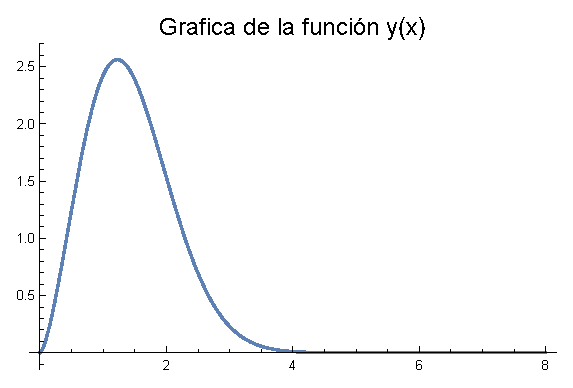
\includegraphics[scale=1]{Imagenes/Plot_Gamma_02_Ejercicio.eps}
\end{figure}

A partir de la figura anterior es claro que la curva se encuentra completamente por encima del eje $x$ positivo con el eje $x$ actuando como una asíntota cuando $x \to \infty$.
\par
Por lo tanto, el área bajo la curva viene dada por la fórmula estándar:
\begin{align*}
A = \scaleint{6ex}_{\bs 0}^{\infty} y \dd{x} = 4 \scaleint{6ex}_{\bs 0}^{\infty} x^{\frac{3}{2}} \, \exp\bigg( -\dfrac{x^{2}}{2} \bigg) \dd{x}
\end{align*}

Haciendo el cambio de variable $t = x^{2} / 2$, se tiene que:
\begin{align*}
A &= 2^{\frac{9}{4}} \scaleint{6ex}_{\bs 0}^{\infty} t^{\frac{1}{4}} \, e^{-t} \dd{t} = \\[0.5em]
&= 2^{\frac{9}{4}} \, \Gamma \bigg( \dfrac{5}{4} \bigg) = \\[0.5em]
&= 4.3116 \hspace{1.5cm} \qed
\end{align*}
\end{ejemplo}
\end{document}
